% !TeX encoding = UTF-8
% !TeX spellcheck = es_ES

\documentclass{DccDiyTools/DccDiyTools}
\usepackage[spanish]{babel}
\usepackage[
type={CC},
modifier={by-sa},
version={4.0},
]{doclicense}


\title{Esquema General}
\author{Daniel Bahn}
\date{Febrero 3}

\dbHeaderTitle{Esquema General}
\dbType{D}
\dbDate{23}
\dbCode{000}
\dbStatus{Draft}
\dbVersion{0.1}

% !TeX encoding = UTF-8
% !TeX spellcheck = es_ES
% !TeX root = ../Esquema.tex
% !TEX root = ../Esquema.tex

\newcommand{\paintBoard}[1][Melon!15]{

    %Base Board
    \draw [fill=#1] (-6,0) rectangle +(3,3)
        (-3,1.5) rectangle +(2,1.5)
        (-1,1.5) rectangle +(2,1.5)
			(1,1.5) rectangle +(2,1.5)
        (6,0) rectangle +(-3,3);
    \draw [fill=Melon!15] (-6,0) rectangle +(3,-3)
        (-3,-1.5) rectangle +(2,-1.5)
        (-1,-1.5) rectangle +(2,-1.5)
        (1,-1.5) rectangle +(2,-1.5)
        (6,0) rectangle +(-3,-3);

}


\newcommand{\paintMain}[2][black]{
    \draw[color=#1,line width=#2] (3,2.1) arc (90:-90:2.1)
    -- (-3,-2.1) arc(-90:-270:2.1) --(3,2.1);
}

\newcommand{\paintStation}[2][black]{
    \draw[color=#1,line width=#2] (5.1,0) --(5.1,-0.3)
        arc(0:-90:2.1) -- (-3,-2.4)
        arc (-90:-180:2.1) -- (-5.1,0);
}

\newcommand{\paintTerminus}[2][black]{
    \draw[color=#1,line width=#2] (-1,-1.8) -- (3,-1.8) arc(-90:90:1.8)
    -- (2.5,1.8) -- (1.2,2.1);

\draw[color=#1,line width=#2] (1.2,-1.8) -- (2.8,-2.1);

}


\newcommand{\paintYard}[2][black]{
	\draw [color=#1,line width=#2] (-2.8,2.1) -- (-1.5,2.4)
		-- (-0.2,2.7);
	\draw [color=#1,line width=#2](-1.5,2.4)
		-- (5,2.4);
	\draw [color=#1,line width=#2](-4,2.7)
		-- (5,2.7);
}



\begin{document}
%\pagestyle{fancy}
\maketitle
\newpage
%\thispagestyle{fancy}
\section{Introduccion}
Daniel Bahn es una empresa ficticia para una maqueta de trenes personal. Esta empresa simula ser la gestora de la red ferroviaria dispuesta en dicha maqueta.
Es por tanto el hilo conductor que nos permite entender dicha maqueta.

Para esta maqueta se ha decidido definir una serie de documentos para llevar el registro y documentacion de la maqueta.
Este documento es el registro del esquema de la maqueta que de manera esquematica es:

\begin{figure}[H]
    \centering

\begin{tikzpicture}

    %\draw [very thin, green]  (-6,-3) grid (6,3);
	\paintBoard  
	\paintMain{2pt}
	\paintStation{2pt}
   \paintTerminus{2pt}
   \paintYard{2pt}
	
\end{tikzpicture}

    \caption{Esquema de la maqueta}
    \label{fig:ModulosBuses}
\end{figure}
\newpage
% !TeX encoding = UTF-8
% !TeX spellcheck = es_ES
% !TeX root = Esquema.tex
% !TEX root = Esquema.tex

\section{Zonas de la maqueta}
El diseño esta basado en la versiones AE y ABC de piko, el nucleo central es la AE, añadiendo una estacion interna y una playa de vias externa. Insipirado en ABC

\begin{figure}[H]
    \centering
	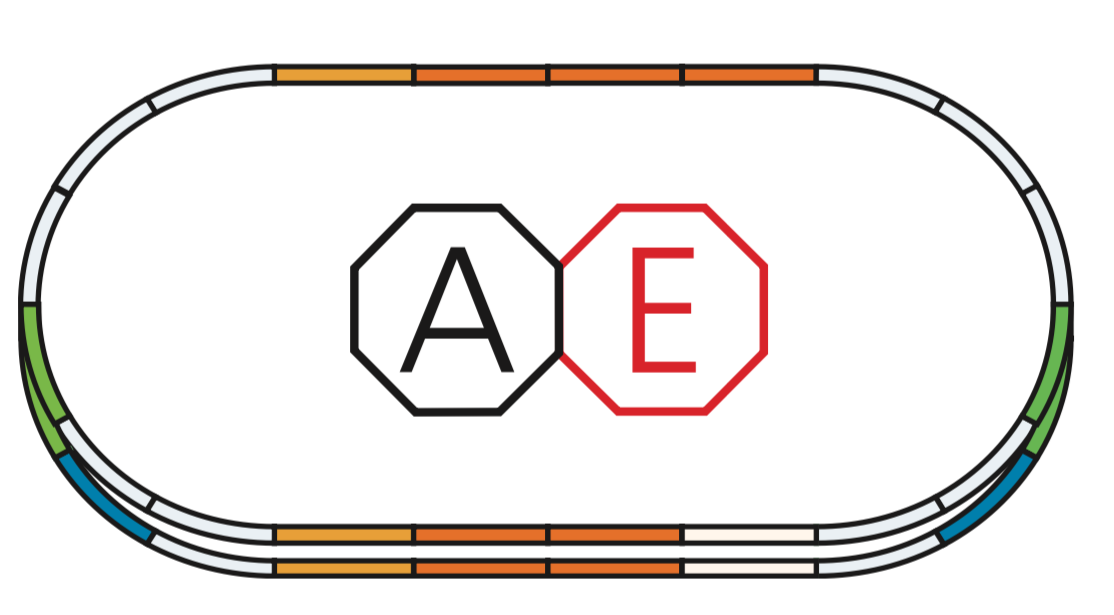
\includegraphics[scale=.25]{Imagenes/PikoAE.png}
   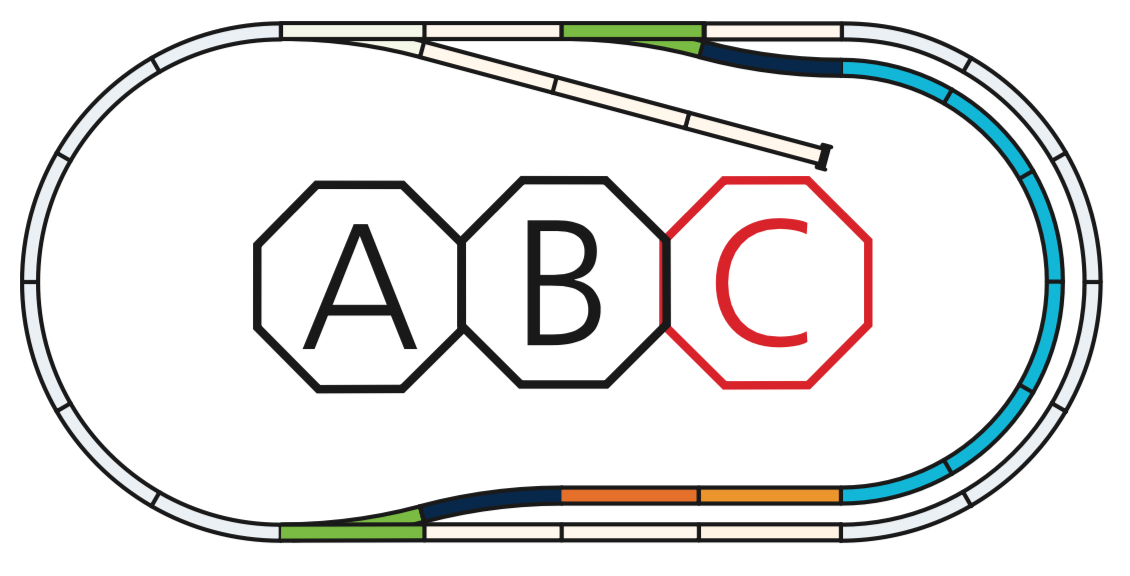
\includegraphics[scale=.25]{Imagenes/PikoABC.png}
    \caption{Inspiracion Original}
    \label{fig:PikoOrigen}
\end{figure}

Asi pues, Daniel Bahn esta organizada 4 Zonas:
\begin{itemize}
\item Linea principal, en negro
\item Estacion, en rojo 
\item Estacion termino, en Verde
\item Playa de vias o Yard, en cyan

\end{itemize}
\begin{figure}[H]
    \centering
\begin{tikzpicture}

    %\draw [very thin, green]  (-6,-3) grid (6,3);
	\paintBoard 
	\paintStation[red]{2pt}
   \paintTerminus[green]{2pt}
   \paintYard[cyan]{2pt}
	  
	\paintMain[black]{4pt}
\end{tikzpicture}

    \caption{Zonas de la maqueta}
    \label{fig:ModulosBuses}
\end{figure}

\subsection{Version Lineal}
Para entender la maqueta pongamosla en una version lineal. Para ello empezarmos antes de la playa de vias y seguiremos la norma de circulacion Oeste a Este\sidenote{Norte en el centro de la maqueta, lo que conlleva un sentido contrario a las agujas del reloj}

\begin{figure}[H]
    \centering
\begin{tikzpicture}
\node[left] at (0,0) {A};

\node[right] at (5,0) {A};

\draw[color=cyan, line width=2pt] (0,-0.5) -- (1.5,-0.5) (1,-.5) -- (1.5,0) (0,-0.25)--(1.25,-0.25);
\draw[color=red,line width=2pt] (2,0)--(2.25,-0.25) -- (3.75,-0.25)--(4,0);

\draw[color=green,line width=2pt] (2.75,0.25)-- (4.25,0.25) -- (4.5,0)
(3.25,0.25) -- (3.5,0) ;
\draw[color=black, line width=4pt] (0,0) -- (5,0);
\end{tikzpicture}

\caption{Version Lineal}
    \label{fig:ModulosBuses}
\end{figure}



\subsection{Extension Virtual}
Esta maqueta se puede extender de una manera ficticia, donde cada zona puede representar diferentes elementos de una red mas grande tras dar una serie vueltas por el ciclo principal.

\begin{figure}[H]
    \centering
\begin{tikzpicture}

\draw[color=cyan, line width=2pt] (6,-0.5) -- (7.5,-0.5) (7,-.5) -- (7.5,0) (6,-0.25)--(7.25,-0.25);

\draw[color=green,line width=2pt] (0,0.25)-- (1.75,0.25) -- (2,0)
(0.75,0.25) -- (1,0) ;

\draw[color=red,line width=2pt](0,-0.25) -- (1.25,-0.25)--(1.5,0) (0,0)--(2.25,0);
\draw[color=red,line width=2pt](0,-0.25) -- (1.25,-0.25)--(1.5,0);
\draw[color=black, line width=4pt] (2.25,0) -- (3,0); 
\node[right](txt) at (3,0) {2 Vueltas};

\draw [color=green,line width=2pt] (5.5,0.25)-- (6.25,0.25) -- (6.5,0);

\draw[color=red,line width=2pt](8.5,0) -- (8.75,-0.25)--(10,-0.25) (8.5,0)--(10,0);


\draw[color=black, line width=4pt] (txt.east) -- (8.5,0);

\end{tikzpicture}

\caption{Version Lineal}
    \label{fig:ModulosBuses}
\end{figure}

En este caso, hemos creado dos estaciones termino, empezamos en la zona <<estacion>> y <<estacion termino>>. Una vez que salimos de la estacion daremos dos vueltas a la via principal.Durante estas dos vueltas ignoraremos los desvios de las zonas <<playa de vias>> y <<estacion termino>>. Pero una vez que hemos dado las dos vueltas la zona <<estacion termino>> repesentara en este caso una linea industrial y justo despues ya tenemos la playa de vias y la estacion final.

No obstante, se documentaran diferentes escenarios en futuros documentos.



\newpage
% !TeX encoding = UTF-8
% !TeX spellcheck = es_ES
% !TeX root = Esquema.tex
% !TEX root = Esquema.tex


\section{Sectores}
Los sectores son las diferentes agrupaciones en las que se divide la maqueta desde unos punto de vista electricos. Los fabricantes suelen llamar a cada una de elementos agruados como \textbf{Districtos} y \textbf{Bloques} \sidenote{Solo para Digital}.

La principal caracterisitica de cada elemento es que esta aislado electricamente del resto\sidenote{En maquetas DC o Analogicas, son conceptos paralelos a cada circutito que puede ser controlado por un mando}. Cada uno de estos elementos (distritos o bloques) va estar precedido por un aparato que conecte dicho elemento a la fuente de energia DCC\sidenote{Ya sea un booster o una central}. La diferencia radica en el objetivo que se quiere obtener con la segmentacion y por lo tanto el dispositivo a conectar. 

\begin{itemize}
\item \textbf{Bloque}: tambien llamado \textit{<<Bloque de deteccion>>}, monitoriza el consumo de corriente y con esa informacion puede inferir si el bloque esta ocupado. 

Puede incluir un detector/lector RailComm y asi poder obtener informacion de la maquina/decoder que esta ocupando el bloque y enviandola al bus LCB.

El bloque debe ser lo más pequeño posible para que solo pueda entrar un elemento a detectar, pero lo suficientemente grande como para detectar el material más grande que se quiera detectar.

\item \textbf{Districto Electrico}: Protege al resto de \textit{districtos} de corto circuitos que puedan exitir en la seccion protegida. El dispositivo conectado controla que el consumo en un   \textit{districto} no supere un cierto umbral, a partir del cual considera que hay un corto y desconecta el distrito de la fuente de potencia.

Hoy en dia las centrales y los booster tienen protecciones ante corto, por lo tanto podria parecer que la division en distritos no es necesaria. Pero si no existen esta particion, un corto, como por ejemplo en la playa de vias, provocaria que toda la maqueta se parara, mientras que con los districtos, en el ejemplo, solo la playa estara sin energia y el resto de la maqueta seguiria funcionando.
\end{itemize}


La maqueta se ha realizado por secciones delimitadas por lo tableros, as 


\begin{figure}[H]
    \centering
\begin{tikzpicture}

    %\draw [very thin, green]  (-6,-3) grid (6,3);
	\paintBoard 

	\paintStation[BlueGreen!25]{5pt}
	\paintMainDb[BlueGreen!25]{5pt}  
	\paintYard[BrickRed!25]{5pt}
	\paintTerminusDb[BlueGreen!25]{5pt}
	
	\paintMainDa[BrickRed!25]{5pt}
	\paintTerminusDa[BrickRed!25]{5pt}
	

	\paintStation[gray]{2pt}
   \paintTerminus[gray]{2pt}
	\paintYard[gray]{2pt}
	\paintMain[gray]{2pt}

	\paintYardZones[cyan!50]{1.5pt}
	\paintMainZones[white]{1.5pt}

	\node[draw=black, text width=4em, line width=1pt](central) at (-8.5,0) {Central Booster};

	\node[draw=black, text width=2em, line width=1pt] (dco1) at (-7,1.5) {DCO};

	\node[draw=black, text width=2em, line width=1pt] (dco2) at (-7,-1.5) {DCO};
	\draw[line width=4pt] (central.east) -- (-7,0)
	-- (dco1.south) -- (dco2.north);

\draw[line width=3pt, BrickRed!25] (dco1.east) -- (-5.5,1.5);
\draw[line width=3pt, BlueGreen!25] (dco2.east) -- (-5.5,-1.5);
	
\end{tikzpicture}

    \caption{Zonas de la maqueta}
    \label{fig:particion}
\end{figure}


\end{document}